% Compile: ./build.sh (Tectonic) or upload the paper/ folder to Overleaf.
% Every number comes from numbers.tex / numbers2.tex, generated by scripts/05_compare.py and 06_extra.py.
\documentclass[10pt,conference]{IEEEtran}
\usepackage{iftex}
\ifXeTeX\usepackage{fontspec}\setmainfont{texgyretermes}[Extension=.otf,UprightFont=*-regular,BoldFont=*-bold,ItalicFont=*-italic,BoldItalicFont=*-bolditalic]\fi
\usepackage{cite}
\usepackage{amsmath}
\usepackage{graphicx}
\usepackage{booktabs}
\usepackage{xcolor}
\usepackage{listings}
\usepackage{tikz}
\usetikzlibrary{positioning,arrows.meta}
\usepackage[hidelinks]{hyperref}
\lstset{basicstyle=\ttfamily\scriptsize,frame=single,framerule=0.3pt,columns=fullflexible,keepspaces=true,aboveskip=3pt,belowskip=6pt,xleftmargin=2pt,xrightmargin=2pt}
% AUTO-GENERATED by scripts/05_compare.py. Do not edit by hand.
\newcommand{\NagentAll}{915}
\newcommand{\NhumanAll}{820}
\newcommand{\Nrepos}{107}
\newcommand{\NagentSame}{462}
\newcommand{\NhumanSame}{631}
\newcommand{\RawAgentPct}{21.4}
\newcommand{\RawHumanPct}{13.3}
\newcommand{\AgentAllPct}{11.7}
\newcommand{\HumanAllPct}{13.8}
\newcommand{\ORAll}{0.71}
\newcommand{\ORloAll}{0.36}
\newcommand{\ORhiAll}{1.37}
\newcommand{\PAll}{0.31}
\newcommand{\PairsAll}{279}
\newcommand{\PairsAAll}{26}
\newcommand{\PairsHAll}{24}
\newcommand{\McPAll}{0.89}
\newcommand{\AgentProdPct}{5.6}
\newcommand{\HumanProdPct}{7.8}
\newcommand{\ORProd}{0.64}
\newcommand{\ORloProd}{0.26}
\newcommand{\ORhiProd}{1.57}
\newcommand{\PProd}{0.33}
\newcommand{\PairsProd}{279}
\newcommand{\PairsAProd}{11}
\newcommand{\PairsHProd}{16}
\newcommand{\McPProd}{0.44}
\newcommand{\AgentHighPct}{5.0}
\newcommand{\HumanHighPct}{6.8}
\newcommand{\ORHigh}{0.65}
\newcommand{\ORloHigh}{0.25}
\newcommand{\ORhiHigh}{1.69}
\newcommand{\PHigh}{0.38}
\newcommand{\PairsHigh}{279}
\newcommand{\PairsAHigh}{10}
\newcommand{\PairsHHigh}{15}
\newcommand{\McPHigh}{0.42}
\newcommand{\ClaudeCodeN}{205}
\newcommand{\ClaudeCodePct}{10.2}
\newcommand{\CodexN}{117}
\newcommand{\CodexPct}{1.7}
\newcommand{\CopilotN}{120}
\newcommand{\CopilotPct}{1.7}
\newcommand{\ORClaude}{1.39}
\newcommand{\ORloClaude}{0.60}
\newcommand{\ORhiClaude}{3.22}
\newcommand{\PClaude}{0.44}
\newcommand{\NClaude}{205}
\newcommand{\PctClaude}{10.2}
\newcommand{\ORCopilot}{0.15}
\newcommand{\ORloCopilot}{0.03}
\newcommand{\ORhiCopilot}{0.93}
\newcommand{\PCopilot}{0.04}
\newcommand{\NCopilot}{120}
\newcommand{\PctCopilot}{1.7}
\newcommand{\ORCodex}{0.15}
\newcommand{\ORloCodex}{0.02}
\newcommand{\ORhiCodex}{1.21}
\newcommand{\PCodex}{0.08}
\newcommand{\NCodex}{117}
\newcommand{\PctCodex}{1.7}
\newcommand{\NTerraform}{519}
\newcommand{\ORTerraform}{0.28}
\newcommand{\PTerraform}{0.13}
\newcommand{\NKube}{579}
\newcommand{\ORKube}{0.89}
\newcommand{\PKube}{0.80}
\newcommand{\TopCat}{identity access}
\newcommand{\TopCatAgent}{3.9}
\newcommand{\TopCatHuman}{6.0}
\newcommand{\MergeAgentClean}{75}
\newcommand{\MergeAgentFind}{50}
\newcommand{\MergeHumanClean}{82}
\newcommand{\MergeHumanFind}{59}
\newcommand{\MergeORFind}{0.38}
\newcommand{\MergePFind}{0.08}
\newcommand{\MergeORlo}{0.13}
\newcommand{\MergeORhi}{1.11}
\newcommand{\MergePInter}{0.99}
\newcommand{\ValN}{110}
\newcommand{\ValPrec}{78}
\newcommand{\NaidevIac}{3,271}
\newcommand{\NaidevRepos}{629}
\newcommand{\NaidevTotal}{361{,}296}
\newcommand{\Nintro}{1,726}
\newcommand{\NhumanCollected}{1,823}
\newcommand{\NhumanRepos}{277}

% AUTO-GENERATED by scripts/06_extra.py
\newcommand{\FixShareA}{4.1}
\newcommand{\NetWorseA}{4.3}
\newcommand{\NetBetterA}{3.0}
\newcommand{\FixShareH}{4.4}
\newcommand{\NetWorseH}{7.0}
\newcommand{\NetBetterH}{3.3}
\newcommand{\ORFix}{0.91}
\newcommand{\PFix}{0.79}
\newcommand{\ORloFix}{0.44}
\newcommand{\ORhiFix}{1.88}
\newcommand{\CommCleanA}{3}
\newcommand{\CommFindA}{4}
\newcommand{\CommCleanH}{2}
\newcommand{\CommFindH}{1}
\newcommand{\IRRComm}{0.54}
\newcommand{\PComm}{0.09}
\newcommand{\NModOnly}{927}
\newcommand{\ORModOnly}{1.06}
\newcommand{\PModOnly}{0.91}
\newcommand{\ORRepoFE}{0.69}
\newcommand{\PRepoFE}{0.51}
\newcommand{\ValFPtest}{24}
\newcommand{\NExamples}{3}
\newcommand{\NagentFetched}{3,249}
\newcommand{\NagentRequested}{3,271}
\newcommand{\NhumanFetched}{1,823}
\newcommand{\NhumanRequested}{1,823}


\begin{document}

\title{Do Coding Agents Widen the Cloud Attack Surface?\\
A Matched Study of Security Misconfigurations in\\ Agent- and Human-Authored Infrastructure-as-Code Changes}

\author{\IEEEauthorblockN{Abhishek Sunil Tiwari}
\IEEEauthorblockA{Independent Researcher, Mumbai, India\\
abhishekst5703@gmail.com}}

\maketitle

\begin{abstract}
AI coding agents now open pull requests that modify Infrastructure-as-Code (IaC), the files that define cloud identities, network exposure and container privileges. Whether these agents introduce security misconfigurations more often than human developers is unknown. We start from the AIDev dataset, identify \NaidevIac{} agent-authored pull requests that change Terraform or Kubernetes files, and obtain \NagentAll{} with scannable configuration. We collect a comparison group of \NhumanAll{} human-authored pull requests from the same repositories. For every pull request we reconstruct each changed file before and after the change and count the security checks that fail only after it. In raw counts, agent pull requests introduce findings more often than human ones (\RawAgentPct\% vs.\ \RawHumanPct\%). Within the same repositories, however, and controlling for change size, we find no significant difference (\NagentSame{} agent vs.\ \NhumanSame{} human pull requests in \Nrepos{} repositories; odds ratio \ORProd, 95\% CI [\ORloProd, \ORhiProd] for misconfigurations in deployable files). The result holds under matched pairs, repository fixed effects, and when only modified files are considered. The apparent gap reflects where agents are used rather than how they write. Agents differ: Claude Code is close to humans, while Copilot and Codex introduce fewer misconfigurations, although these per-agent differences do not survive correction for multiple comparisons. Agents also fix existing misconfigurations about as often as humans. Pull requests that introduce a deployable misconfiguration tend to be merged less often for both groups, yet they rarely attract more review discussion. Our results caution against judging agent security from repository-level counts and point to automated checks in code review as the practical control for agent-written cloud configuration.
\end{abstract}

\begin{IEEEkeywords}
infrastructure as code, coding agents, security misconfiguration, Terraform, Kubernetes, mining software repositories, empirical software engineering
\end{IEEEkeywords}

\section{Introduction}
Infrastructure-as-Code (IaC) turns cloud configuration into versioned source files. A Terraform module or a Kubernetes manifest decides which identities may perform which actions, which services are reachable from the internet, and with which privileges containers run. A single line can grant an identity unrestricted permissions or run a container that can escalate to the host. Studies of open-source IaC have repeatedly found such security smells and misconfigurations~\cite{rahman2019sins,rahman2021ansible,rahman2023k8s}, including in widely reused Helm charts~\cite{zerouali2023helm,minna2025helm}.

At the same time, autonomous coding agents such as Claude Code, GitHub Copilot's coding agent, OpenAI Codex, Devin and Cursor have moved from suggesting lines to opening complete pull requests. Adoption on GitHub is rapid~\cite{robbes2026agentic}, and the AIDev dataset records hundreds of thousands of agent-authored pull requests~\cite{li2026aidev}. Agents are increasingly asked to edit IaC: Barrak et al.\ found that agent IaC pull requests are larger than human ones and more often modify core infrastructure, while introducing maintainability smells at a similar rate~\cite{barrak2026agents}.

Related work gives reasons for concern. Agent pull requests often contain security smells~\cite{sakib2026trust}; models struggle to infer least-privilege permissions~\cite{yan2026leastpriv}; and LLM ``fixes'' to Terraform misconfigurations often satisfy the scanner without removing the risk~\cite{alsaid2026terraprobe}. None of these studies measures whether agent-written changes to cloud configuration introduce misconfigurations at a different rate than comparable human changes. The answer matters: if agents systematically weaken cloud configuration, teams need agent-specific guardrails; if they do not, effort should go to the review process that both agents and humans pass through.

A fair comparison is not straightforward. Agents are not used uniformly: they are concentrated in particular repositories and tasks. Repository-level counts therefore mix the effect of the author with the effect of the project. We address this with a within-repository, size-adjusted design that attributes each misconfiguration to the pull request that introduced it, and we ask:
\begin{itemize}
  \item \textbf{RQ1 (Prevalence):} Do agent-authored IaC pull requests introduce security misconfigurations more often than human-authored ones?
  \item \textbf{RQ2 (Categories):} Which kinds of misconfiguration do agents and humans introduce?
  \item \textbf{RQ3 (Review and net effect):} Are misconfiguration-introducing pull requests merged and discussed, and do agents also fix misconfigurations?
\end{itemize}

\noindent\textbf{Findings in brief.} (1) Raw counts suggest agents are worse (\RawAgentPct\% vs.\ \RawHumanPct\% of pull requests introduce a finding), but within the same repositories there is no significant difference (OR \ORProd; Section~\ref{sec:rq1}). (2) Agents differ from one another by an order of magnitude. (3) The categories introduced by agents mirror those introduced by humans, led by identity and access issues. (4) Misconfiguration-introducing changes tend to be merged less often for both groups but are not discussed more in review.

\noindent\textbf{Contributions.} (i)~The first security-focused, within-repository comparison of agent- and human-authored IaC changes, covering \NaidevIac{} candidate agent pull requests from AIDev; (ii)~evidence of a repository-context confound that future studies of agent output must control for; (iii)~per-agent estimates, category profiles and real examples of agent-introduced misconfigurations; (iv)~an open, change-level measurement pipeline and replication package.

\section{Background}
\subsection{Infrastructure as Code and Misconfiguration}
Terraform describes cloud resources (identities, networks, storage) in HashiCorp Configuration Language; Kubernetes manifests describe workloads, their containers and their privileges in YAML. Both are typically changed through pull requests and reviewed like application code. Static analysers such as Checkov evaluate these files against hundreds of policy checks, for example that an IAM policy does not grant actions on all resources (\texttt{"*"}), that a container cannot escalate privileges, or that storage is not publicly accessible. Because the checks are rule-based, a finding indicates that a risky setting is present, not that it is exploitable in context; our validation step (Section~\ref{sec:validation}) addresses this.

\subsection{Coding Agents and the AIDev Dataset}
Coding agents receive a task, edit a repository and open a pull request, often with little human editing. AIDev collects such pull requests from public GitHub repositories together with their commits, file-level changes and review events~\cite{li2026aidev}. Its curated subset, which we use, contains \NaidevTotal{} pull requests labelled by agent.

\section{Related Work}
\textbf{Security of IaC.} Rahman et al.\ catalogued security smells in Puppet scripts~\cite{rahman2019sins} and in Ansible and Chef scripts~\cite{rahman2021ansible}, and studied security misconfigurations in open-source Kubernetes manifests~\cite{rahman2023k8s}. GLITCH generalised smell detection across IaC languages~\cite{saavedra2022glitch}, and Chiari et al.\ surveyed static analysis for IaC~\cite{chiari2022survey}. Helm charts have been analysed for outdatedness and security risks~\cite{zerouali2023helm} and for misconfigurations and their LLM-assisted mitigation~\cite{minna2025helm}. Eom et al.\ benchmarked Kubernetes misconfiguration scanners and documented disagreements between them~\cite{eom2026scanners}.

\textbf{Coding agents on GitHub.} Robbes et al.\ measured agent adoption from the traces agents leave in commits and pull requests~\cite{robbes2026agentic}. Li et al.\ released AIDev~\cite{li2026aidev}. Barrak et al.\ compared agent, bot and human IaC pull requests, their acceptance and their maintainability smells~\cite{barrak2026agents}.

\textbf{Security of agent output.} Sakib et al.\ characterised security smells in agent-generated pull requests across general code~\cite{sakib2026trust}. Yan et al.\ evaluated whether coding agents infer least-privilege permissions~\cite{yan2026leastpriv}. Alsaid et al.\ showed that LLM repairs of Terraform misconfigurations are frequently deceptive~\cite{alsaid2026terraprobe}. Least privilege for cloud functions has also been studied directly~\cite{sankaran2020iam,shin2026alps}.

\textbf{Positioning.} Table~\ref{tab:positioning} summarises the closest studies. Prior IaC security work analyses repository snapshots of human-written code; prior agent work studies either maintainability or general code. Ours is, to our knowledge, the first to compare agent and human changes to cloud configuration for security within the same repositories.

\begin{table}[t]
\centering
\caption{Closest prior studies and how this study differs.}
\label{tab:positioning}
\footnotesize
\begin{tabular}{@{}p{2.1cm}p{1.6cm}p{1.6cm}p{1.9cm}@{}}
\toprule
Study & Artefact & Authors & Outcome \\
\midrule
Rahman et al.~\cite{rahman2019sins,rahman2021ansible} & Puppet, Ansible, Chef scripts & Humans & Security smells \\
Rahman et al.~\cite{rahman2023k8s} & K8s manifests & Humans & Misconfigurations \\
Minna et al.~\cite{minna2025helm} & Helm charts & Humans & Misconfigurations \\
Barrak et al.~\cite{barrak2026agents} & IaC PRs & Agents vs.\ humans & Maintainability smells \\
Sakib et al.~\cite{sakib2026trust} & General PRs & Agents & Security smells \\
\textbf{This study} & TF + K8s PRs & Agents vs.\ humans, same repos & Security misconfigs, merge, fixes \\
\bottomrule
\end{tabular}
\end{table}

\section{Study Design}
Fig.~\ref{fig:pipeline} summarises the pipeline. All scripts are released (Section~\ref{sec:data}).

\begin{figure*}[t]
\centering
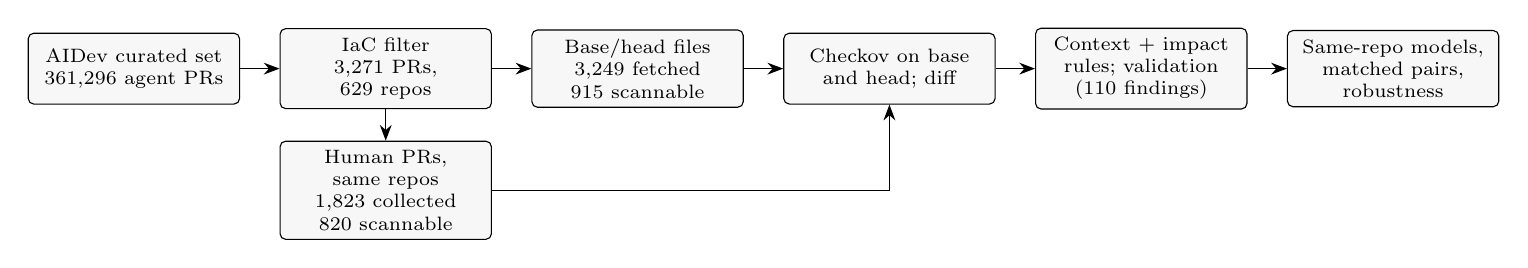
\begin{tikzpicture}[node distance=4mm and 5mm, every node/.style={font=\scriptsize}, box/.style={draw, rounded corners=2pt, align=center, minimum height=9mm, text width=2.45cm, fill=gray!6}, arr/.style={-{Stealth[length=2mm]}}]
\node[box] (a) {AIDev curated set\\\NaidevTotal{} agent PRs};
\node[box, right=of a] (b) {IaC filter\\\NaidevIac{} PRs, \NaidevRepos{} repos};
\node[box, right=of b] (c) {Base/head files\\\NagentFetched{} fetched\\\NagentAll{} scannable};
\node[box, below=of b] (h) {Human PRs, same repos\\\NhumanCollected{} collected\\\NhumanAll{} scannable};
\node[box, right=of c] (d) {Checkov on base\\and head; diff};
\node[box, right=of d] (e) {Context + impact\\rules; validation\\(\ValN{} findings)};
\node[box, right=of e] (f) {Same-repo models,\\matched pairs,\\robustness};
\draw[arr] (a) -- (b); \draw[arr] (b) -- (c); \draw[arr] (c) -- (d); \draw[arr] (d) -- (e); \draw[arr] (e) -- (f);
\draw[arr] (b) -- (h); \draw[arr] (h.east) -| (d.south);
\end{tikzpicture}
\caption{Study pipeline. Agent pull requests come from AIDev; human pull requests come from the same repositories. Every pull request is scanned before and after the change.}
\label{fig:pipeline}
\end{figure*}

\subsection{Agent Pull Requests}
From AIDev's curated subset we selected pull requests changing at least one Terraform file (\texttt{.tf}, \texttt{.tfvars}) or a YAML file under a Kubernetes-related path, reading only file-name columns of the commit-detail table. This yielded \NaidevIac{} pull requests in \NaidevRepos{} repositories, created between January 2025 and March 2026. For each, we retrieved base and head commits and changed files from the GitHub API (\NagentFetched{} available) and downloaded every changed IaC file at both commits. We kept Kubernetes YAML only if it was a plain manifest (containing \texttt{apiVersion} and \texttt{kind} and no template expressions): Helm templates require rendering and are excluded. This left \NagentAll{} agent pull requests with scannable configuration.

\subsection{Human Comparison Group}
For each repository we collected merged or closed pull requests created within 180 days of that repository's agent pull requests and changing the same file types, up to 25 per repository. We excluded any pull request listed in AIDev, authored by a bot account, or carrying agent traces in its description or recent commit messages (e.g., ``Generated with Claude Code'', agent co-author trailers). This yielded \NhumanCollected{} human pull requests in \NhumanRepos{} repositories; the same download and filtering left \NhumanAll{} with scannable configuration.

\subsection{Measuring Introduced Misconfigurations}
We ran Checkov (Terraform and Kubernetes frameworks) separately on the base and head versions of each pull request's files. A finding is \emph{introduced} if a check fails for a resource at head but not at base, and \emph{fixed} if it fails at base but not at head. We map each check to one of eleven categories by its name (Table~\ref{tab:checks} lists the most frequent checks). Findings in test fixtures, examples and similar paths are marked \emph{non-deployable}; checks whose violation can directly enable access, privilege escalation, exposure or data leakage are marked \emph{high-impact}. We report three binary outcomes per pull request: any introduced finding, any introduced finding in a deployable file (our primary outcome), and any high-impact finding in a deployable file.

\subsection{Validation}\label{sec:validation}
We drew a stratified random sample of \ValN{} introduced findings (at most one per pull request) with the author group hidden from the rater. Each finding was labelled a real problem in deployable configuration or a false alarm. Labels were first proposed with the context rules above and then reviewed by the author, who agreed with all of them; the labelled sample is released with the replication package. Overall, \ValPrec\% of sampled findings were real problems (Table~\ref{tab:validation}); the \ValFPtest{} false alarms all came from test fixtures, examples and scanner test cases, which the deployable-file outcome excludes.

\begin{table}[t]\centering\caption{Manual validation: share of sampled introduced findings that are real problems in deployable configuration.}\label{tab:validation}\small\begin{tabular}{@{}lrr@{}}\toprule Subset & Findings & Real\\\midrule
All sampled findings & 110 & 78\% \\
High-impact checks & 52 & 77\% \\
Hygiene checks & 58 & 79\% \\
Terraform files & 34 & 68\% \\
Kubernetes files & 76 & 83\% \\
\bottomrule\end{tabular}\end{table}


\subsection{Analysis}
We restrict comparisons to the \Nrepos{} repositories containing both agent and human pull requests (Table~\ref{tab:dataset}). For each outcome we fit a logistic regression on author type and the logarithm of IaC lines added, with standard errors clustered by repository. As a design-based check, we pair each agent pull request with the human pull request of nearest size in the same repository (without replacement) and apply McNemar's exact test. Robustness checks use repository fixed effects and restrict to pull requests that modify existing files. Per-agent comparisons use a Bonferroni-corrected threshold ($\alpha=0.017$ for three agents). For RQ3 we model merging with an author-by-outcome interaction, and review comments with a negative binomial model.

\begin{table}[t]\centering\caption{Matched sample: pull requests (PRs), repositories, IaC types, median IaC lines added, and merge rate.}\label{tab:dataset}\small\begin{tabular}{@{}lrrrrrr@{}}\toprule Author & PRs & Repos & TF & K8s & Lines & Merged\\\midrule
Claude Code & 205 & 65 & 86 & 119 & 24 & 74\% \\
Copilot & 120 & 42 & 80 & 40 & 45 & 64\% \\
Codex & 117 & 11 & 73 & 45 & 25 & 91\% \\
Other agents & 20 & 4 & 0 & 20 & 78 & 25\% \\
\midrule
All agents & 462 & 107 & 239 & 224 & 27 & 74\% \\
Humans & 631 & 107 & 280 & 355 & 17 & 80\% \\
\bottomrule\end{tabular}\end{table}


\section{Results}
\subsection{RQ1: Prevalence}\label{sec:rq1}
Across all scannable pull requests, \RawAgentPct\% of agent and \RawHumanPct\% of human pull requests introduce at least one finding. Within the same repositories the difference disappears (Table~\ref{tab:rq1}). For deployable files, \AgentProdPct\% of agent and \HumanProdPct\% of human pull requests introduce a misconfiguration (OR \ORProd, 95\% CI [\ORloProd, \ORhiProd], $p=\PProd$). The matched-pair analysis agrees: of \PairsProd{} pairs, \PairsAProd{} have a finding only in the agent change and \PairsHProd{} only in the human change (McNemar $p=\McPProd$).

\begin{table}[t]
\centering
\caption{Share of pull requests introducing at least one finding, same repositories. OR: odds ratio for agent vs.\ human, adjusted for change size, repository-clustered 95\% CI.}
\label{tab:rq1}
\small
\begin{tabular}{@{}lccc@{}}
\toprule
Outcome & Agent & Human & OR [95\% CI] \\
\midrule
Any finding & \AgentAllPct\% & \HumanAllPct\% & \ORAll{} [\ORloAll, \ORhiAll] \\
Deployable file & \AgentProdPct\% & \HumanProdPct\% & \ORProd{} [\ORloProd, \ORhiProd] \\
High-impact, deployable & \AgentHighPct\% & \HumanHighPct\% & \ORHigh{} [\ORloHigh, \ORhiHigh] \\
\bottomrule
\end{tabular}
\end{table}

\textbf{Why the raw gap disappears.} Agent pull requests are concentrated in repositories with more IaC activity and tend to be larger (Fig.~\ref{fig:size}); once we compare pull requests from the same repositories and adjust for size, author type no longer predicts misconfigurations.

\textbf{Robustness.} The result is stable: with repository fixed effects (OR \ORRepoFE, $p=\PRepoFE$), restricted to the \NModOnly{} pull requests that modify existing files (OR \ORModOnly, $p=\PModOnly$), for Terraform (OR \ORTerraform, $p=\PTerraform$) and for Kubernetes (OR \ORKube, $p=\PKube$).

\begin{figure}[t]
\centering
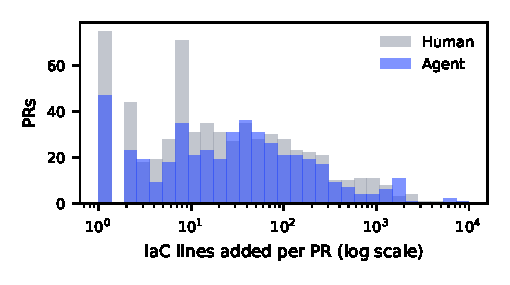
\includegraphics[width=\columnwidth]{fig_size.pdf}
\caption{IaC lines added per pull request, matched repositories.}
\label{fig:size}
\end{figure}

\textbf{Agents differ.} Compared with humans in the same repositories (Fig.~\ref{fig:agents}), Claude Code shows no significant difference (\PctClaude\% of \NClaude{} pull requests; OR \ORClaude{} [\ORloClaude, \ORhiClaude], $p=\PClaude$), whereas Copilot (\PctCopilot\% of \NCopilot; OR \ORCopilot{} [\ORloCopilot, \ORhiCopilot], $p=\PCopilot$) and Codex (\PctCodex\% of \NCodex; OR \ORCodex{} [\ORloCodex, \ORhiCodex], $p=\PCodex$) introduce fewer deployable misconfigurations. None of these differences remains significant after Bonferroni correction; we report them as signals for future work.

\begin{figure}[t]
\centering
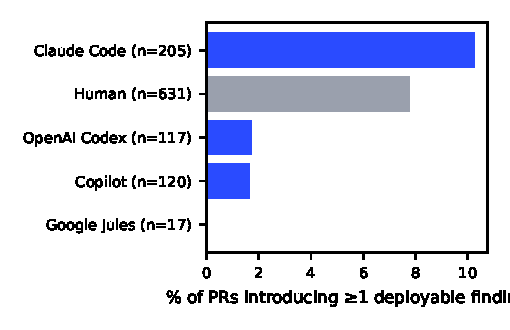
\includegraphics[width=\columnwidth]{fig_agents.pdf}
\caption{Pull requests introducing at least one misconfiguration in a deployable file, by author (same repositories; authors with at least ten pull requests).}
\label{fig:agents}
\end{figure}

\begin{figure}[t]
\centering
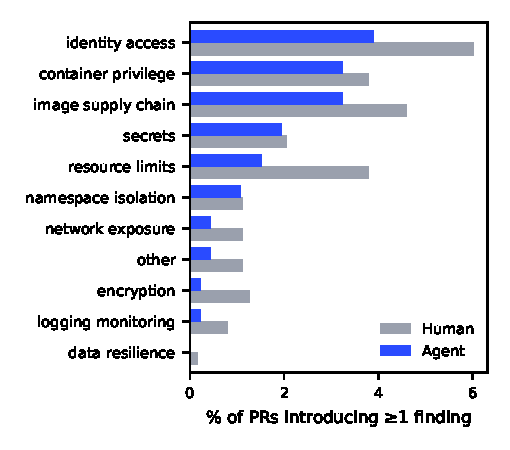
\includegraphics[width=\columnwidth]{fig_categories.pdf}
\caption{Share of pull requests introducing each category of misconfiguration in deployable files (same repositories).}
\label{fig:cats}
\end{figure}

\subsection{RQ2: Categories}
Fig.~\ref{fig:cats} breaks deployable findings down by category, and Table~\ref{tab:checks} lists the most frequent checks. The leading category for agents is \TopCat{} (\TopCatAgent\% of agent vs.\ \TopCatHuman\% of human pull requests), followed by container privilege and image supply chain. Agent rates do not exceed human rates in any category, indicating no agent-specific weakness. The profile nevertheless matches the concerns raised by prior work on least privilege and container security~\cite{yan2026leastpriv,rahman2023k8s}.

\begin{table}[t]\centering\caption{Most frequent checks introduced in deployable files: number (\%) of agent and human PRs introducing each.}\label{tab:checks}\footnotesize\begin{tabular}{@{}p{5.1cm}rr@{}}\toprule Check (Checkov name) & Agent & Human\\\midrule
Ensure that Service Account Tokens are only mounted where nece… & 12 (2.6) & 23 (3.6) \\
Containers should run as a high UID to avoid host conflict & 12 (2.6) & 23 (3.6) \\
Ensure that the seccomp profile is set to docker/default or ru… & 13 (2.8) & 21 (3.3) \\
Image should use digest & 12 (2.6) & 21 (3.3) \\
Use read-only filesystem for containers where possible & 13 (2.8) & 19 (3.0) \\
Minimize the admission of root containers & 9 (1.9) & 19 (3.0) \\
Apply security context to your pods and containers & 8 (1.7) & 19 (3.0) \\
Minimize the admission of containers with capabilities assigne… & 9 (1.9) & 18 (2.9) \\
Minimize the admission of containers with the NET\_RAW capabili… & 9 (1.9) & 18 (2.9) \\
Image Pull Policy should be Always & 8 (1.7) & 19 (3.0) \\
\bottomrule\end{tabular}\end{table}


The following real agent-introduced findings from deployable files in our sample illustrate these categories (excerpts of the head version): a wildcard IAM resource, a container without a security context, and a storage account without a public-access restriction.

\noindent\textit{Example 1} (Claude Code, \texttt{iam.tf}): Ensure no IAM policies documents allow "*" as a statement's resource for restrictable actions.
\begin{lstlisting}
data "aws_iam_policy_document" "ab_tag_policy_document" {
  count = local.create_iam_resources ? 1 : 0
  statement {
    effect    = "Allow"
    resources = ["*"]
    actions = [
      "backup:ListTags",
      "backup:TagResource",
      "backup:UntagResource",
\end{lstlisting}

\noindent\textit{Example 2} (Claude Code, \texttt{deployment.yaml}): Containers should not run with allowPrivilegeEscalation.
\begin{lstlisting}
      containers:
        - name: cockroach
          image: cockroachdb/cockroach:latest-v24.2
          command: ["cockroach"]
          args: ["start-single-node", "--insecure"]
          ports:
            - name: sql
              containerPort: 26257
            - name: http
\end{lstlisting}

\noindent\textit{Example 3} (Claude Code, \texttt{staticweb.tf}): Ensure that Storage accounts disallow public access.
\begin{lstlisting}
resource "azurerm_storage_account" "staticweb" {
  name                             = local.staticweb_storage_name
  resource_group_name              = var.resource_group_name
  location                         = var.location
  account_kind                     = "StorageV2"
  account_tier                     = "Standard"
  account_replication_type         = "LRS"
  table_encryption_key_type        = var.enable_cmk_encryption ? "Acco
  queue_encryption_key_type        = var.enable_cmk_encryption ? "Acco
\end{lstlisting}


\subsection{RQ3: Review, Merge and Net Effect}
\textbf{Merging.} Pull requests that introduce a deployable misconfiguration are merged less often: \MergeHumanClean\% vs.\ \MergeHumanFind\% for humans and \MergeAgentClean\% vs.\ \MergeAgentFind\% for agents. After adjusting for size and author type, the association is in the same direction but not significant at the 5\% level (OR \MergeORFind, 95\% CI [\MergeORlo, \MergeORhi], $p=\MergePFind$), and it does not differ between agents and humans (interaction $p=\MergePInter$).

\textbf{Discussion in review.} Misconfiguration-introducing pull requests do not attract more comments (median \CommFindA{} vs.\ \CommCleanA{} for agents, \CommFindH{} vs.\ \CommCleanH{} for humans; rate ratio \IRRComm, $p=\PComm$). Where these changes are filtered, it is apparently not through explicit security discussion.

\textbf{Net effect.} Agents also remove misconfigurations: \FixShareA\% of agent and \FixShareH\% of human pull requests fix at least one existing finding (OR \ORFix{} [\ORloFix, \ORhiFix], $p=\PFix$). \NetWorseA\% of agent pull requests leave configuration with more findings than before and \NetBetterA\% with fewer, compared with \NetWorseH\% and \NetBetterH\% for humans.

\section{Discussion}
\textbf{For researchers: control for repository context.} Without matching, agents look substantially worse; with matching they do not. Agent usage is concentrated in particular projects and tasks, so pooled comparisons across repositories risk attributing project differences to the agent. We recommend within-repository designs and reporting results per agent, since estimates differ by an order of magnitude between agents.

\textbf{For practitioners: automate the check.} Agents and humans introduce misconfigurations at similar rates, and these changes are not discussed more in review. Running an IaC scanner on every pull request, regardless of author, is therefore a more effective control than treating agent changes as uniquely risky.

\textbf{For agent builders: scan before opening a pull request.} Agents still introduce high-impact misconfigurations in \AgentHighPct\% of matched pull requests, most often wildcard permissions and missing container security contexts. Running a scanner on the diff before opening a pull request, and requesting least-privilege defaults, is a cheap mitigation.

\section{Threats to Validity}
\textbf{Construct validity.} Undisclosed agent use cannot be detected, so some ``human'' pull requests may be agent-assisted, which biases results toward no difference. Scanner findings include false alarms; our validation and the deployable-file outcome address the main source (test and example files). Category and impact labels are rule-based.
\textbf{Internal validity.} Agents may receive different tasks than humans; same-repository, size-adjusted comparisons and repository fixed effects reduce but do not remove this. Scanning only changed files can miss cross-file context. Merging and commenting have many causes besides security.
\textbf{External validity.} We study public repositories in AIDev, a subset of agents and a fixed period; Helm templates are excluded; private and enterprise repositories may differ.
\textbf{Conclusion validity.} The matched sample is modest, so confidence intervals are wide and small differences cannot be ruled out; per-agent tests are corrected for multiplicity.

\section{Ethical Considerations}
We analysed only public repositories and public pull requests. We did not contact developers, run code from the studied repositories, or interact with deployed systems. We report results in aggregate and do not identify individual developers; released data contains repository and pull-request identifiers only, without author names or account details.

\section{Conclusion}
In a within-repository comparison, AI coding agents did not introduce cloud security misconfigurations more often than human developers, although raw counts suggest they do. Agents differ from one another, fix existing misconfigurations about as often as humans, and their misconfiguration-introducing changes, like human ones, tend to be merged less often but are not discussed more in review. Future work should render Helm charts, follow merged misconfigurations into later commits, and extend the study to more agents and to private repositories.

\section*{Data Availability}\label{sec:data}
Scripts, pull-request identifiers, scanner outputs and the validation sample are available at \url{https://github.com/abhishek572003/iac-agent-security}.

\section*{Use of AI Tools}
The author used an AI assistant (Anthropic's Claude) for programming support, literature search and verification, and language editing. All data collection, analyses and results were produced by the released scripts and checked by the author, who takes full responsibility for the content.

\bibliographystyle{IEEEtran}
\bibliography{refs}
\end{document}
